\chapter{Ley de acción de masas}

Ahora dejamos los puentes y cambiamos a otro tipo de modelos totalmente diferentes. Vamos a hablar de la ley de acción de masas, pero primero vamos a repasar un poco algunas nociones sobre reacciones químicas. Tenemos una serie de productos $A_1,\cdots, A_n$, $B_1,\cdots, B_n$ y una serie de coeficientes que nos indican la concentración de cada producto: $\alpha_1,\cdots, \alpha_n$, $\beta_1,\cdots, \beta_n$. A estos coeficientes se les llama \textit{coeficientes estequiométricos}. Estos elementos nos dan una reacción química, que expresaremos como:
\[
\alpha_1A_1+\cdots+\alpha_nA_n \longrightarrow \beta_1B_1+\cdots+\beta_nB_n
\]
\begin{example} La reacción química de la quema de hidrógeno:
\[
2H_2+0_2\longrightarrow 2H_20
\]
Otra diferente:
\[
ClH+NaOH \longrightarrow ClNa+H_20
\]
\end{example}

Esto es una cuestión molecular y trabajar con ellas es bastante complicado. Para solventar ese problema, usamos los \textit{moles}. Un \textit{mol} es la cantidad de una sustancia que contiene tantos átomos como su peso atómico. También usaremos la \textit{concentración de un producto}, $[N]$, que es el igual al número de moles que hay del producto. En la reacción anterior obtendríamos dos moles de agua, combinando dos moles de hidrógeno y un mol de oxígeno. Podemos hablar de concentración de \textit{reactivos} y \textit{productos}: $[A] = \{ \text{ número de moles de reactivo } \}$, $[B] = \{ \text{ número de moles de producto } \}$

Por otro lado, está la denominada \textit{velocidad de reacción}, que es la variación de la concentración a lo largo del tiempo. La teoría nos dice que:
\[
\frac{d}{dt}[B]=k[A_1]\cdots[A_n]
\]

\section{Reacción química}

Sean $X,Y$ y $Z$ tre compuestos químicos que se combinan en un producto final $F$ según la reacción:
\[
2X+3Y+5Z\longrightarrow 5F
\]
La velocidad de reacción (moléculas más o menos iguales) se puede suponer proporcional al producto de concentraciones de productos $X,Y,Z$, según un coeficiente $\beta$ (velocidad de reacción). Suponemos que $\beta=0.01$. Si partimos inicalmente de 5 moles de $X$, 7 moles de $Y$ y 10 moles de $Z$, plantear un modelo que permita calcular la concentración de cada sustancia en cada instante. ¿Qué pasará tras mucho tiempo?

Básicamente hay que aplicar una regla de 3:
\[
\left.
\begin{array}{ccc}
2X & \longrightarrow & 5F\\
5X & \longrightarrow & ?
\end{array}
\right\} \Rightarrow \text{ se producirían  12.5F}
\]
\[
\left.
\begin{array}{ccc}
3Y & \longrightarrow & 5F\\
7Y & \longrightarrow & ? = 
\end{array}
\right\} \Rightarrow \text{ se producirían  11.6F }
\]
\[
\left.
\begin{array}{ccc}
5Z & \longrightarrow & 5F\\
10Z & \longrightarrow & ? = 10 
\end{array}
\right\} \Rightarrow \text{ se producirían  10F }
\]
De aquí, deduzco que se van a producir 10 moles de $F$, ya que es el mínimo de las 3 reglas que hemos hecho. Ahora tenemos que ver cuanta cantidad queda de los reactivas $X$ e $Y$ al crear 10 moles de $F$.
\[
\left.
\begin{array}{ccc}
2X & \longrightarrow & 5F\\
? & \longrightarrow & 10F
\end{array} 
\right\}
\Rightarrow \text{ se gastan 4X }
\]
\[
\left.
\begin{array}{ccc}
3Y & \longrightarrow & 5F\\
? & \longrightarrow & 10F
\end{array}
\right\} \Rightarrow \text{ se gastan 6Y }
\]
Luego sobran 1 de $X$, 1 de $Y$ y 0 de $Z$, y se habrán creado 10 moles de $F$. Ahora vamos a denotar por $x(t),y(t),z(t),F(t)$ a la concentración de $X,Y,Z,F$ en el instante $t$ respectivamente. En el instante $t=0$, tendremos las concentraciones iniciales, y en el instante $t=1$, tendremos las finales (el resultado de las cuentas que hemos hecho antes), es decir:
\[
\begin{array}{|c|c|c|}
\hline
& t=0 & t=1 \\
\hline
x(t) & 4 & 1\\
\hline
y(t) & 7 & 1\\
\hline
z(t) & 10 & 1\\
\hline
F(t) & 0 & 1\\
\hline
\end{array}
\]
Si nos fijamos, $5-x(t),7-y(t),10-z(t)$ son los restantes de los productos $X,Y,Z$ en el instante $t$. Es decir, tenemos que la velocidad de reacción de $F$ es:
\[
F'(t)=\beta x(t)y(t)z(t)
\]
Haciendo otra regla de 3:
\[
\left.
\begin{array}{ccc}
2X & \longrightarrow & 5F\\
5-x(t) & \longrightarrow & F(t)
\end{array}
\right\} \Rightarrow F(t)=\frac{5(5-x(t))}{2} \Rightarrow x(t)=5-\frac{2F(t)}{5}
\]
De forma análoga, obtenemos las expresiones de $y(t)$ y $z(t)$:
\[
y(t)=7-\frac{3F(t)}{5}, \espacio z(t)=10-F(t)
\]
Es decir, la expresión final de la velocidad de reacción sería:
\[
F'(t)=0.01\left(5-\frac{2F(t)}{5}\right)\left(7-\frac{3F(t)}{5}\right)\left(10-F(t)\right), \espacio F(0)=0
\]

Si llamamos $g(F)=0.01\left(5-\frac{2F}{5}\right)\left(7-\frac{3F}{5}\right)\left(10-F\right)$, que tiene raíces $F=10,35/3,12.5$. 

\begin{center}
\begin{tikzpicture}[scale=0.5]
\draw (0,0) -- (16,0);
% parabola
\draw[scale=1,domain=0:16,smooth,variable=\x,red] plot ({\x}, {0.01*(5-2*\x/5)*(7-3*\x)*(10-\x)});

% etiquetas
\draw[dashed] (2.3,-0.7) -- (2.3,.2);
\draw (2.3,-1) node[anchor=north] {$10$};
\draw[dashed] (10,-0.7) -- (10,.2);
\draw (10,-1) node[anchor=north] {$\frac{35}{3}$};
\draw[dashed] (12.7,-0.7) -- (12.7,.2);
\draw (12.7,-1) node[anchor=north] {$12.5$};

\draw (2,2) node[] {$g(F)$};

\end{tikzpicture}
\end{center}

Ahora vamos a abstraer un poco el problema para no tener que trabajar con todos los números particulares. Supongamos que tenemos el problema de valores iniciales:
\[
\left\{
\begin{array}{l}
x'=g(x) \\
x(0)=x_0, \espacio x_0<\alpha_1
\end{array}
\right.
\]
donde $\funcion{g}{\R}{\R}$, $g(\alpha_1)=0$, $g'(\alpha_1)<0$ (para que sea compatible con el dibujo), $g(x)>0$ si $x\in(-\infty, \alpha_1)$ y $\alpha_1$ es la primera raíz de $g$. 

Como sabemos, el anterior problema de valores iniciales tiene una solución maximal $\funcion{x}{(w_-,w_+)}{\R}$, que además es única. Probemos ahora una serie de propiedades.
\begin{itemize}
\item $x(t)<\alpha_1, \text{ si } t\in(w_-,w_+)$

Tomamos $t^*\in(w_-,w_+)$ con $x(t^*)=\alpha_1$, entonces $x$ sería solución del problema de valores iniciales:
\[
\left\{
\begin{array}{l}
x'=g(x) \\
x(t^*)=\alpha_1
\end{array}
\right.
\]
cuya solución es la constante, $x(t)=\alpha_1$ $\forall t\in(w_-,w_+)$. (\textbf{duda: no entiendo esta demostracion x'd})

\item $x'(t)>0$ $\forall t\in(w_-,w_+)$

Usando el punto anterior es fácil, ya que $x'(t)=g(x(t))>0$ porque $g(x)$ es positivo para todo $x$ en $(-\infty, \alpha_1)$

\item Necesariamente se tiene que $w_+=+\infty$.

Si $t\in[0,w_+)$, entonces $x_0\leq x(t) < \alpha_1$. Ahora podemos usar la teoría de prolongación de soluciones, que nos dice que si tenemos una solución acotada, podemos prolongarla. $x$ además de estar acotada, está lejos del borde. 

\item $\limitemasinfinito{t}{x(t)}=\alpha_1$

Como $x(t)$ es creciente y acotada, entonces el límite existe, y valdrá $L\in\R$. Evidentemente, $L\leq \alpha_1$. Lo único que tenemos que ver es que $L=\alpha_1$. Para ello, vamos a recordar un resultado general:
\begin{lemma}
Sea $\funcion{x}{(w_-,+\infty)}{\R}\in\mathcal{C}^1$ con $\limitemasinfinito{t}{x(t)}=L\in\R$. Entonces existe una sucesión $t_n\in(w_-,+\infty)$ tal que $t_n\longrightarrow +\infty$, con $x'(t_n)\longrightarrow 0$.
\end{lemma}
\begin{proof}
Considerando la diferencia $x(n+1)-x(n)$ y aplicando el teorema del valor medio, nos queda que:
\[
x(n+1)-x(n)=x'(t_n)(n+1-n)=x'(t_n)
\]
Como $x(n+1)\longrightarrow L \leftarrow x(n)$, $x'(t_n)\longrightarrow 0$.
\end{proof}
Luego al existir el límite anterior, existe también $t_n\longrightarrow +\infty$ tal que $x'(t_n)\longrightarrow 0$, es decir, $g(x(t_n))\longrightarrow 0$.  Pero $g(x(t_n))\longrightarrow g(L)$, luego $L=\alpha_1$, que es la raíz.
\end{itemize}

Como $\alpha_1$ era la primera raíz de $g$, es decir, $\alpha_1=10$, hemos visto que $F(t)\longrightarrow 10$. Pero ojo, simplemente tiende, nunca llegamos a crear los 10 moles enteros, es una asíntota que no se alcanza en tiempo finito. Además $F(t)<10$ $\forall t \in(0,+\infty)$.

Usando la cota sobre $F(t)$ y recordando la expresión de $x(t)$, llegamos a que:
\[
x(t)=5-\frac{2F(t)}{5}>5-4=1 \Rightarrow x(t)\longrightarrow 1
\]
Igual con la $y(t)$ y $z(t)$:
\[
y(t)=7-\frac{3F(t)}{5}>7-6=1 \Rightarrow y(t)\longrightarrow 1
\]
\[
z(t)=10-F(t) \Rightarrow z(t)\longrightarrow 0
\]

Volvemos otra vez a la parte abstracta. Sea $g\in\mathcal{C}^2$ de la forma:

\begin{center}
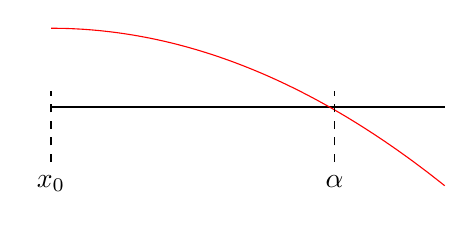
\begin{tikzpicture}
\draw (0,0) -- (5,0);
% parabola
\draw[scale=1,domain=0:5,smooth,variable=\x,red] plot ({\x}, {-0.08*\x*\x+1});

% etiquetas
\draw[dashed] (0,-0.7) -- (0,.2);
\draw (0,-0.75) node[anchor=north] {$x_0$};
\draw[dashed] (3.6,-0.7) -- (3.6,.2);
\draw (3.6,-0.75) node[anchor=north] {$\alpha$};
\end{tikzpicture}
\end{center}

cumpliendo $g(\alpha)=0$ y $g'(\alpha)=\delta<0$. Entonces vamos a tener que (lo que he visto antes):
\[
\limitemasinfinito{t}{x(t)}=\alpha
\]
Ahora vamos a decir un poquito más. Vamos a probar que:
\[
\limitemasinfinito{t}{\frac{x(t)-\alpha}{e^{\delta t}}}=L\in(-\infty,0)
\]
Eso quiere decir que la convergencia al valor $\alpha$ es exponencial, es decir, los residuos ($x(t),y(t),z(t))$ no sólo tienden a (1,1,0), sino que además lo hacen exponencialmente.
\begin{proof}
Calculemos el siguiente límite:
\[
\limitemasinfinito{t}{\frac{x'(t)}{x(t)-\alpha}}=\limitemasinfinito{t}\frac{g(x(t))}{x(t)-\alpha}=\limite{x}{\alpha}{\frac{g(x)}{x-\alpha}}=\delta
\]
Eso nos dice que si tenemos $\beta(t)=\frac{x'(t)}{x(t)-\alpha}$, entonces $\beta(t)\longrightarrow \delta$. Por supuesto, $\beta$ es continua y se verifica la ecuación diferencial:
\[
x'(t)= \beta(t)(x(t)-\alpha)
\]
Usando que $x(t)=\alpha$ es una solución particular de esa ecuación y $x(t)=ce^{-\int_0^t\beta(t)dt}$ es una solución de la homogénea, podemos escribir la solución general:
\[
x(t)=\alpha-ce^{-\int_0^t\beta(t)dt}
\]
donde hemos añadido la solución de la homogénea directamente restando porque sabemos que se tiene que cumplir $x(t)<\alpha$. Diviendo todo por $e^{\delta t}$:
\[
\frac{x(t)-\alpha}{e^{\delta t}}=\frac{-ce^{-\int_0^t\beta(t)dt}}{e^{\delta t}}=-ce^{-\int_0^t\beta(t)dt-\delta t}=-ce^{-\int_0^t\left(\beta(s)-\delta \right)ds}
\]
Ahora ya lo único que queda por ver es que $\beta(s)-\delta$ sea integrable en $(0,+\infty)$. Para eso:
\[
\beta(t)-\delta=\frac{x'(t)}{x(t)-\alpha}-\delta=\frac{g(x(t))-\delta(x(t)-\alpha)}{x(t)-\alpha}=\frac{g(x)-g(\alpha)-g'(\alpha)(x-\alpha) }{x-\alpha}\leq O(x-\alpha)
\]
donde para la acotación por algo de orden $x-\alpha$ hemos usado que $g\in\mathcal{C}^2$, luego:
\[
\beta(t)-\delta\leq O(x(t)-\alpha)
\]
%================================= corrección
Para ver que $x(t)-\alpha$ es integrable, se puede expresar $g(x(t))$ de la siguiente forma:
\[
g(x(t))=\frac{x(t)-\alpha}{g(x(t))}x'(t)
\]
Se vió anteriormente que el primer término converge a una constante ($-\frac{1}{\delta}$), luego solo hay que comprobar si $x'(t)$ es integrable. Como $x'(t)>0$, se tiene:
\[
\integral{0}{+\infty}{x'(t)dt}=\limitemasinfinito{T}{\integral{0}{T}{x'(t)dt}}=
\limitemasinfinito{T}{\left(x(T)-x(0)\right)}=\alpha-x(0)
\]
Luego $x'$ es integrable (lebesgue) en $(0,+\infty)$.
%=================================
\end{proof}

Este es el único modelo que vamos a desarrollar con este nivel de detalle, los siguientes serán más escuetos.

\section{Reacción química en equilibrio}
%================================== clase 27/05

En este modelo se supone que hay dos sustancias químicas, $A$ y $B$, con concentraciones $\alpha$ y $\beta$ respectivamente. Estas dos sustancias químicas se combinarán para forma una tercera sutancia, $C$, con concentración $\gamma$. La diferencia de este modelo con el anterior, es que en este se va a considerar posible que parte del producto $C$, vuelva a descomponerse en las sustancias $A$ y$B$. Esa nueva reacción química se va a represenar como sigue:
\[
\alpha A + \beta B \underset{k_{-1}}{\overset{k_1}{\rightleftarrows}} \gamma C
\]
donde $k_1$ y $k_{-1}$ son constantes. Se denota por $x(t),y(t)$ y $z(t)$  al número de moles de $A$,$B$ y $C$ respectivamente, y por $a_0$, $b_0$ a las cantidades iniciales de $A$ y $B$. La cantidad inicial de $C$ se supone 0.

Al igual que antes, si se hace una regla de tres con los productos $A$ y $C$ se obtiene:
\[
\left.
\begin{array}{ccc}
\alpha A & \longrightarrow & \gamma C\\
a_0-x(t) & \longrightarrow & z(t)
\end{array}
\right\} \Rightarrow z(t)=\frac{(a_0-x(t))\gamma}{\alpha}
\]
\[
\left.
\begin{array}{ccc}
\beta B & \longrightarrow & \gamma C\\
b_0-y(t) & \longrightarrow & z(t)
\end{array}
\right\} \Rightarrow z(t)=\frac{(b_0-y(t))\gamma}{\beta}
\]
Además, la variación de concentado tiene como expresión: $z'(t)=k_1x(t)y(t)$. Ojo, esto solo es para la reacción hacia la derecha. También se debe tener en cuenta la relación hacia la izquierda, en la que se destruyen moléculas de $C$ según la constante $k_{-1}$. $z'$ quedaría entonces:
\[
z'(t)=k_1x(t)y(t)-k_{-1}z(t)
\]
Despejando de las reglas de tres del principio, se obtienen las expresiones de $x(t)$ y $y(t)$, quedando:
\[
z'(t)=k_1\left(a_0-\frac{\alpha z(t)}{\gamma}\right)\left(b_0-\frac{\beta z(t)}{\gamma}\right)-k_ {-1}z(t)
\]
Al igual que en el otro modelo, se toma $z'=g(z)$ para estudiar la ecuación. Se ve que el primer término de $g$ es una parábola, con dos raíces diferentes dependientes de $\alpha$ y $\beta$. El segundo es una recta de pendiente $k_{-1}$ que corta a esa parábola.

\textbf{duda: me no sale una parábola invertida}

\begin{center}
\begin{tikzpicture}[scale=1]
\draw (-1,0) -- (5,0);
 parabola
\draw[scale=1,domain=-1:5,smooth,variable=\x,red] plot ({\x}, {0.5*(1-\x)*(1-\x)-\x});
\draw[scale=1,domain=-1:5,smooth,variable=\x,blue] plot ({\x}, {0.3*\x-0.3});

\draw[dashed] (4.2,-0.35) -- (4.2,1.1);
\draw (4.3,-0.35) node[anchor=north] {$z^*$};
\end{tikzpicture}
\end{center}
$z^*$ es la raíz más grande de las dos que salen al resolver $g(z)=0$. Eso implica que $z(t)\longrightarrow z^*$. Se toma tombién $x^*$ e $y^*$ como el resultado de despejar $x(t)$ e $y(t)$ al sustituir $z(t)$ por $z^*$ en las expresiones anteriores. Como $z^*$ es raíz de $g$, queda:
\[
k_1x^*y^*=k_{-1}z^*
\]
A partir de esa expresión se deduce la ley de \textit{equilibrio químico}:
\[
\frac{x^*y^*}{z^*}=\frac{k_{-1}}{k_1}
\]
%==================================

%================================== 28/05

\section{Modelo de Michaelis-Menten (1913)}

Se supone una especie de \textit{bacteria}, con el núcleo (en negro) y la membrana citoplasmática. Dentro de esa membrana, hay una serie de enzimas, cuyo único objetivo es coger los nutrientes e introducirlos dentro de la misma.

\begin{center}
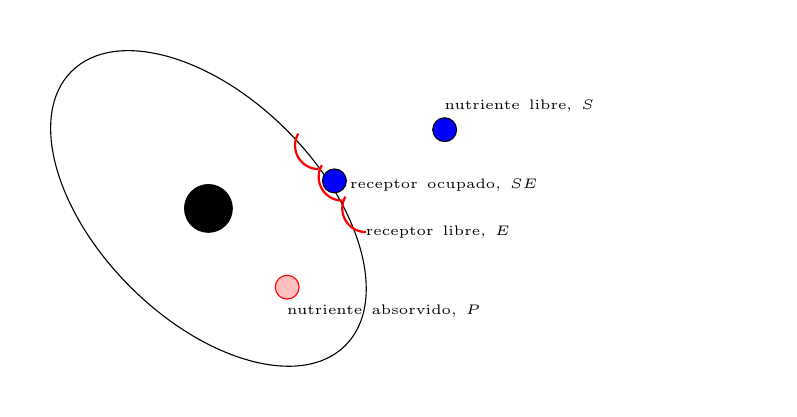
\begin{tikzpicture}[scale=1]
% celula
\draw[rotate=45] (0,0) ellipse (40pt and 70pt);
\draw[black,fill=black] (0,0) circle (2ex);
% nutrientes
\node[text width=4cm] at (3,-1.3) {\tiny nutriente absorvido, $P$};
\draw[red,fill=pink] (1,-1) circle (1ex);
\node[text width=4cm] at (5,1.3) {\tiny nutriente libre, $S$};
\draw[fill=blue] (3,1) circle (1ex);
\node[text width=4cm] at (3.8,0.3) {\tiny receptor ocupado, $SE$};
\draw[fill=blue] (1.6,0.35) circle (1ex);
% receptores
\draw [red,thick,domain=150:270] plot ({2+0.3*cos(\x)}, {0.3*sin(\x)});
\draw [red,thick,domain=150:270] plot ({1.7+0.3*cos(\x)}, {0.4+0.3*sin(\x)});
\node[text width=4cm] at (4,-0.3) {\tiny receptor libre, $E$};
\draw [red,thick,domain=150:270] plot ({1.4+0.3*cos(\x)}, {0.8+0.3*sin(\x)});
\end{tikzpicture}
\end{center}

Este intercambio de nutrientes se puede representar por la siguiente reacción química:
\[
\ce{S + E <=>[k_1][k_{-1}] SE ->[k_2] E + P } 
\]
Si un nutriente libre es atrapado por un receptor, se tiene un receptor ocupado (con constante $k_1$). Este proceso puede deshacerse, es decir, un receptor ocupado puede soltar el nutriente que tenga (esta reacción pasa con constante $k_{-1}$). Si la obsorción tiene éxito, entonces el nutriente se absorve y el receptor vuelve a quedar libre (esto pasa con constante $k_2$). 

Se denota por:
\begin{itemize}
\item $s(t)$: cantidad de nutrientes libres.
\item $e(t)$: concentración de encimas libres.
\item $c(t)$: concentración de encimas ocupadas.
\item $p(t)$: concentración de nutrientes absorvidos.
\end{itemize}

El objetivo es escribir y estudiar la ecuación diferencial que sigue este modelo. Al principio, una parte del sustrato reacciona con la enzima, disminuyendo la cantidad de nutrientes libres, luego se añade $-k_1s(t)e(t)$. Pero como este enlace se puede romper, liberando esos nutrientes, también hay que añadir: $k_{-1}c(t)$. Luego:
\[
s'(t)=-k_1s(t)e(t)+k_{-1}c(t)
\]
De igual forma se razona con $e'(t)$:
\[
e'(t)=k_2c(t)+k_{-1}c(t)-k_1s(t)e(t)
\]
donde el primer término es la concentración de receptores que se quedan libres al producirse la absorción, el segundo son los liberados por escape del nutriente y el último son los que pasan a estar ocupados.

Repitiendo el razonamiento, se obtienen las dos ecuaciones restantes:
\[
\begin{array}{l}
c'(t)=k_1s(t)e(t)-k_{-1}c(t)-k_2c(t)\\
p'(t)=k_2c(t)
\end{array}
\]
En resumen, se tienen cuatro ecuaciones diferenciales distintas:
\[
\left\{
\begin{array}{l}
s'(t)=-k_1s(t)e(t)+k_{-1}c(t)\\
e'(t)=\left(k_2+k_{-1}\right)c(t)-k_1s(t)e(t)\\
c'(t)=k_1s(t)e(t)-\left(k_{-1}+k_2\right)c(t)\\
p'(t)=k_2c(t)
\end{array}
\right.
\]
Al sumar la segunda y tercera ecuación, se obtiene que $e'(t)+c'(t)=0$, es decir, el número de enzimas en la membrana es constante, obviamente. Se tiene que la concentración de nutrientes también es constante (sumando la primera y las dos últimas). Estos dos valores se representan por las constantes $T_e$ y $T_n$, respectivamente. Además, si se integra en las dos sumas:
\[
\begin{array}{l}
T_e=e(t)+c(t)\\
T_n=s(t)+c(t)+p(t)
\end{array}
\]
Ya se tiene el planteamiento del problema, ahora se necesitan los datos iniciales. Se supone que hay nutrientes tanto fuera de la célula como dentro. Además de que en el momento 0 ya hay receptores ocupados y libres, es decir:
\[
s(0)=s_0>0, \espacio e(0)=e_0, \espacio c(0)=c_0, \espacio p(0)=p_0, \espacio T_e=e_0+c_0>0
\]
Para los siguientes razonamientos se deja de lado la última ecuación (la de $p'(t)$), porque al depender solo de $c(t)$ no va a ser de mucha ayuda en este estudio.

Tomando las dos primeras ecuaciones y sustituyendo $c(t)=T_e-e(t)$ queda:
\[
\left\{
\begin{array}{l}
s'(t)=-k_1s(t)e(t)+k_{-1}(T_e-e(t))\\
e'(t)=\left(k_2+k_{-1}\right)(T_e-e(t))-k_1s(t)e(t)\\
\end{array}
\right.
\]
Que es un sistema de dos ecuaciones diferenciales. Se supone que se tiene una solución maximal $\funcion{s,e}{(w_-,w_+)}{\R}$ y se prueban varias propiedades, que hacen que el modelo tenga sentido:
\begin{itemize}
\item $e(t)>0$ $\forall t\in[0,w_+)$

Se tiene que $e(0)=e_0\geq 0$. Si $e_0=0$, entonces $e'(0)=(k_{-1}+k_2)T_e>0$, por lo tanto: $e(t)>0$ en un intervalo $(0,\varepsilon)$.

Si $e_0>0$, existe $\varepsilon>0$ tal que $e(t)>0$ en el intervalo $(0,\varepsilon)$. Por reducción al absurdo, se supone que existe $\bar{t}\in[0,w_+)$ de forma que $e(\bar{t})<0$. Sea $t^*=\inf\{t\in[0,w_+]:e(t)<0\}$. De ahí se deduce que $e(t^*)=0$, puesto que antes de $t^*$, $e(t)$ es positivo y después de $t^*$ es negativo. Al ser $e(t^*)=0$, queda $e'(t^*)=(k_{-1}+k_2)T_e>0$.

\item $e(t)<T_e$ $\forall t\in(0,w_+)$. Este apartado se prueba de forma análoga al anterior. (\textbf{completar})
\item $s(t)>0$ $\forall t \in[0,w_+)$. Este apartado se prueba de forma análoga al anterior. (\textbf{completar})
\end{itemize}

Volviendo al sistema de ecuciones general, sean $\funcion{s,e,c,p}{[0,w_+)}{\R}$ son solcuciones maximales. Se ha visto que $s(t)$ y $e(t)$ son positivas. $c(t)$ también lo es ya que se puede expresar como $c(t)=T_e-e(t)$, que siempre es positivo ya que $e(t)<T_e$ para todo $t$.

La expresión $s(t)+e(t)+p(t)=T_n$ indica que todas las soluciones están acotadas por $T_n$, luego la teoría de prolongación de soluciones nos dice que podemos prolongarla hasta el infinito, es decir, $w_+=+\infty$.

\subsection{Comportamiento asintótico}

Ahora se va a proceder al estudio del comportamiento asintótico de estas soluciones. Se tienen dos sistemas (en el apartado anterior se dejó la $p$ aparte):
\[
\left\{
\begin{array}{l}
s'(t)=-k_1s(t)e(t)+k_{-1}c(t)\\
e'(t)=\left(k_2+k_{-1}\right)c(t)-k_1s(t)e(t)\\
c'(t)=k_1s(t)e(t)-\left(k_{-1}+k_2\right)c(t)\\
\end{array}
\right.
\left\{
\begin{array}{l}
p(t)=T_n-c(t)-s(t)\\
p'(t)=k_2c(t)
\end{array}
\right.
\]
El primer sistema se puede ver como la ecuación diferencial $x'=f(x)$ donde $\funcion{f}{\R^3}{\R^3}$, $f\in\mathcal{C}^{1}$ y $x(t)$ es una solución acotada para $t\geq 0$.

Para demostrar eso se necesita el teorema de \textit{Lasalle}, que requiere mucha terminología. Aquí se va a usar una adpatación. Sea $\funcion{V}{\R^2}{\R}$ una función definida por $V(s,c)=s+c$ y se denota por $\dot{V}(s,c)=\frac{d}{dt}V(s(t),c(t))=-k_{-1}c$ a su derivada. Como $\dot{V}(s,c)\leq 0$, se tiene que $V$ es una función guía de ese problema.
\medskip
\begin{theorem}[Teorema de Lassale (adaptación)]
Sea $V\funcion{V}{\R^N}{\R}$. Si $V(x(t))$ es decreciente (función de Liapunov) y $x(t)$ está positivamente acotada, entonces $\dot{V}(x(t))\longrightarrow 0$.
\end{theorem}

Luego si se aplica ese teorema a este caso, tenemos que $\dot{V}(x(t))=-k_{-1}c(t)\longrightarrow 0$, por lo tanto, $c(t)\longrightarrow 0$. Como se tenía que $T_e=e(t)+c(t)$, lo anterior implica que $e(t)\longrightarrow T_e$. Esto quiere decir que las enzimas tienden a quedarse todas libres, ya que se ha visto que las ocupadas tienden a 0. 

Además $p(t)$ tiene límite por ser una función acotada y creciente. Con $s(t)$ pasa exactamente lo mismo, $s(t)=T_n-c(t)-p(t)$ y $s(t)\longrightarrow s^*$.

\begin{lemma}
Si $\funcion{s}{[0,+\infty)}{\R}$ es de clase 1 y existe su límite, es decir:
\[
\limitemasinfinito{t}{s(t)\in\R}
\]
Entonces $t_n\longrightarrow+\infty$ con $s'(t_n)\longrightarrow 0$.
\end{lemma}

Aplicando ese lema a $s(t)$, se tiene que:
\[
s'(t_n)=k_{-1}c(t_n)-k_1s(t_n)e(t_n)
\]
Haciendo ahora $t_n\longrightarrow +\infty$, se obtiene que $s^*T_e=0$. Como $T_e\neq 0$, tiene que ser $s^*=0$ t por lo tanto $p(t)\longrightarrow T_n$.

En definitiva se ha visto que las concentraciones tienden a:
\[
\left\{
\begin{array}{l}
s(t)\longrightarrow 0\\
e(t)\longrightarrow T_e\\
c(t)\longrightarrow 0\\
p(t)\longrightarrow T_n
\end{array}
\right.
\]
Lo que significa que todas las enzimas se quedan libres después de haber absorvido todos los nutrientes disponibles.

%================================== 

%================================== 29/05

%================================== 
